% !TeX program = xelatex
\documentclass[UTF8]{beamer}

% -----------------------------------------------------------------------------
% Language, typography, mathematics, tables, and graphics
% -----------------------------------------------------------------------------
\usepackage{xeCJK}
\usepackage{amsmath}
\usepackage{physics}
\usepackage{booktabs}
\usepackage{tabularx}
\usepackage{graphicx}
\usepackage{xcolor}
\usepackage{tcolorbox}
\tcbuselibrary{skins}

% Preserve the project presentation typography.
\usepackage[T1]{fontenc}
\usepackage{palatino}
\setCJKmainfont{Noto Serif CJK SC}
\setCJKsansfont{Noto Serif CJK SC}
\setCJKmonofont{Noto Serif CJK SC}
\setmonofont{Inconsolata}
\def\mathfamilydefault{\rmdefault}

% 16:9 slide canvas from the reusable Durham/Stanford template.
\usepackage[
  orientation=landscape,
  size=custom,
  width=16,
  height=9,
  scale=0.5
]{beamerposter}

% Compatibility fix for older Babel releases.
\makeatletter
\let\@@magyar@captionfix\relax
\makeatother

% -----------------------------------------------------------------------------
% Theme and deck-specific visual language
% -----------------------------------------------------------------------------
\usetheme{Stanford}
\beamertemplatenavigationsymbolsempty
\setbeamerfont{frametitle}{size=\Large,series=\bfseries}
\setbeamerfont{title}{size=\LARGE,series=\bfseries}
\setbeamercolor{itemize item}{fg=darkcyan}
\setbeamercolor{itemize subitem}{fg=darkcyan}

\definecolor{bdmblue}{RGB}{29,78,121}
\definecolor{bdmteal}{RGB}{0,124,146}
\definecolor{bdmgreen}{RGB}{0,128,96}
\definecolor{bdmgold}{RGB}{188,122,25}
\definecolor{bdmrose}{RGB}{174,63,79}
\definecolor{bdmred}{RGB}{158,42,43}
\definecolor{bdmpale}{RGB}{244,247,249}

\newtcolorbox{phasebox}[2][]{%
  enhanced,
  colback=white,
  colframe=#2,
  boxrule=1.2pt,
  arc=1.5mm,
  left=1.6mm,
  right=1.6mm,
  top=0.9mm,
  bottom=0.9mm,
  before upper={\raggedright},
  #1
}

\newcommand{\metric}[3]{%
  \begin{tcolorbox}[
    enhanced,
    colback=#1!7,
    colframe=#1,
    boxrule=1.0pt,
    arc=1.2mm,
    left=1.8mm,
    right=1.8mm,
    top=0.7mm,
    bottom=0.7mm,
    before upper={\raggedright}
  ]
    {\color{#1}\bfseries\large #2}\hspace{1.0ex}{\footnotesize #3}
  \end{tcolorbox}%
}

\newcommand{\source}[1]{}

% -----------------------------------------------------------------------------
% Presentation metadata
% -----------------------------------------------------------------------------
\title[BDM Session 3]{\textbf{BDM Session 3}}
\subtitle{Correctness, convergence, and the evidence-gated path to validated physics}

\author[C.-Z. Ruan]{\Large Cheng-Zong Ruan}

\institute[Durham University]{%
  
\includegraphics[height=0.72in]{durham_logo.png}\\[0.65ex]
  \small Institute for Computational Cosmology, Durham University
}
\date{27 August 2026}

% -----------------------------------------------------------------------------
% Document
% -----------------------------------------------------------------------------
\begin{document}

\begin{frame}[plain]
  \titlepage
\end{frame}

\begin{frame}{The campaign was gated before it was scaled}
  \footnotesize
  \begin{columns}[T,totalwidth=\textwidth]
    \begin{column}{0.318\textwidth}
      \begin{phasebox}{bdmblue}
        {\color{bdmblue}\bfseries\large 3A --- Correctness}\par\smallskip
        Minimal safety patch only\\[0.5ex]
        Immutable legacy/corrected baselines\\[0.5ex]
        Synthetic, Fortran, identity, resource gates\par\smallskip
        {\bfseries Outcome:} corrected numerical baseline green
      \end{phasebox}
    \end{column}
    \hfill
    \begin{column}{0.318\textwidth}
      \begin{phasebox}{bdmteal}
        {\color{bdmteal}\bfseries\large 3B --- Finder + sampling}\par\smallskip
        OFAT first; compact design frozen second\\[0.5ex]
        Same immutable state for finder variants\\[0.5ex]
        Nested and independent ID selections\par\smallskip
        {\bfseries Outcome:} GO for bounded GR calibration
      \end{phasebox}
    \end{column}
    \hfill
    \begin{column}{0.318\textwidth}
      \begin{phasebox}{bdmgold}
        {\color{bdmgold}\bfseries\large 3C --- End to end}\par\smallskip
        Matched-phase particle and force scans\\[0.5ex]
        Finder mesh deconfounded from force mesh\\[0.5ex]
        Compact joint design; no Cartesian product\par\smallskip
        {\bfseries Outcome:} bounded design closed; science NO-GO
      \end{phasebox}
    \end{column}
  \end{columns}

  \vfill

  \begin{phasebox}[colback=bdmpale,top=1.0mm,bottom=1.0mm]{coolgray}
    \centering
    \textbf{Session 3C footprint:}
    22 new GR simulations $\vert$ 23 physical states analysed $\vert$
    135 terminal Slurm allocations $\vert$ 49.12 billed core-hours\\[0.5ex]
    All ICs used validated FML 2LPTIC at $z_{\rm ini}=49$ with stable uint64 IDs;
    all light work ran on \texttt{cosma8-serial}.
  \end{phasebox}
  \source{Frozen evidence: \texttt{results/bdm\_convergence/manifest.json}}
\end{frame}

\begin{frame}{The corrected finder is numerically reproducible}
  \footnotesize
  \begin{columns}[T,totalwidth=\textwidth]
    \begin{column}{0.54\textwidth}
      \begin{phasebox}{bdmblue}
        {\color{bdmblue}\bfseries Minimal Session 3 safety corrections}\par\smallskip
        \begin{itemize}\setlength\itemsep{0.15em}
          \item Read and validate configuration before density or peak work
          \item Replace the raced fixed maxima buffer with stable compaction
          \item Emit a valid empty catalogue when there are zero maxima
          \item Use the declared snapshot background density
          \item Guard shape, $V_{\max}$, $R_{\max}$, roots, and denominators
          \item Record exact integer $N_{\rm bound}$ in an opt-in sidecar
        \end{itemize}
      \end{phasebox}

      \vspace{0ex}
      \centering\footnotesize\color{bdmgreen}
      \textbf{Production physics, defaults, and legacy \texttt{Catshort}
      are unchanged.}
    \end{column}
    \hfill
    \begin{column}{0.42\textwidth}
      \metric{bdmgreen}{21/21}{final login-safe + real-Fortran tests pass}
      \metric{bdmteal}{0}{repeat/thread representation floor}
      \metric{bdmblue}{1--128}{OpenMP thread counts are byte-identical}
      \metric{bdmgold}{fast = precise}{candidate sets and downstream propagation}
      \begin{phasebox}[colback=white,top=0.8mm,bottom=0.8mm]{coolgray}
        \footnotesize
        Archived production executable unchanged:\par
        \texttt{c84f4e3c\ldots ad89}
      \end{phasebox}
    \end{column}
  \end{columns}
  \source{Final verification SHA-256: \texttt{1c996658\ldots04a76}}
\end{frame}

\begin{frame}{Finder sampling is not converged by 500 particles}
  \footnotesize
  \begin{columns}[T,totalwidth=\textwidth]
    \begin{column}{0.64\textwidth}
      \centering
      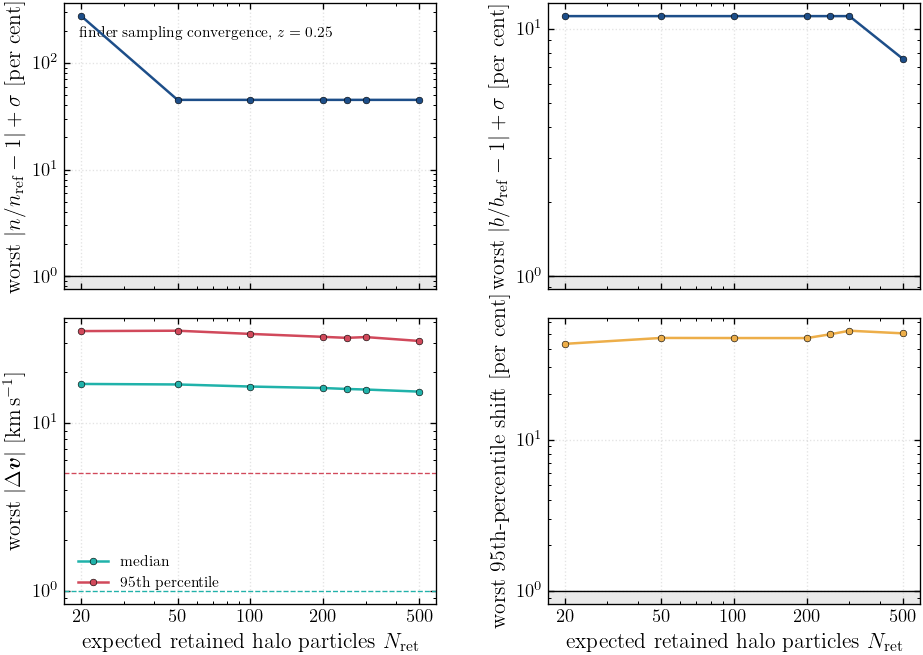
\includegraphics[width=\linewidth,height=0.56\textheight,keepaspectratio]{figs/sampling_thresholds.png}
    \end{column}
    \hfill
    \begin{column}{0.33\textwidth}
      \begin{phasebox}{bdmrose}
        {\color{bdmrose}\bfseries At the 500-particle cut}\par\smallskip
        \scriptsize
        \begin{tabularx}{\linewidth}{@{}Xr@{}}
          HMF shift $+$ error & $45.0\%$ \\[0.3ex]
          clustering shift $+$ error & $7.54\%$ \\[0.3ex]
          velocity median & $15.36\,\mathrm{km\,s^{-1}}$ \\[0.3ex]
          velocity p95 & $30.77\,\mathrm{km\,s^{-1}}$ \\[0.3ex]
          internal-property p95 & $50.4\%$ \\
        \end{tabularx}
      \end{phasebox}

      \vspace{0.3ex}
      \begin{phasebox}[colback=bdmgold!8,top=0.8mm,bottom=0.8mm]{bdmgold}
        \centering
        \textbf{All application thresholds remain unresolved above 500}
      \end{phasebox}

      \vspace{0.3ex}
      \scriptsize
      Stable-ID construction passes. Label: \textbf{finder sampling convergence},
      not simulation-resolution convergence.
    \end{column}
  \end{columns}
  \source{Session 3B controlled-sampling analysis; thresholds were not extrapolated}
\end{frame}

\begin{frame}{Particle, force, and finder-mesh resolution are all sensitive}
  \small
  \begin{columns}[T,totalwidth=\textwidth]
    \begin{column}{0.64\textwidth}
      \centering
      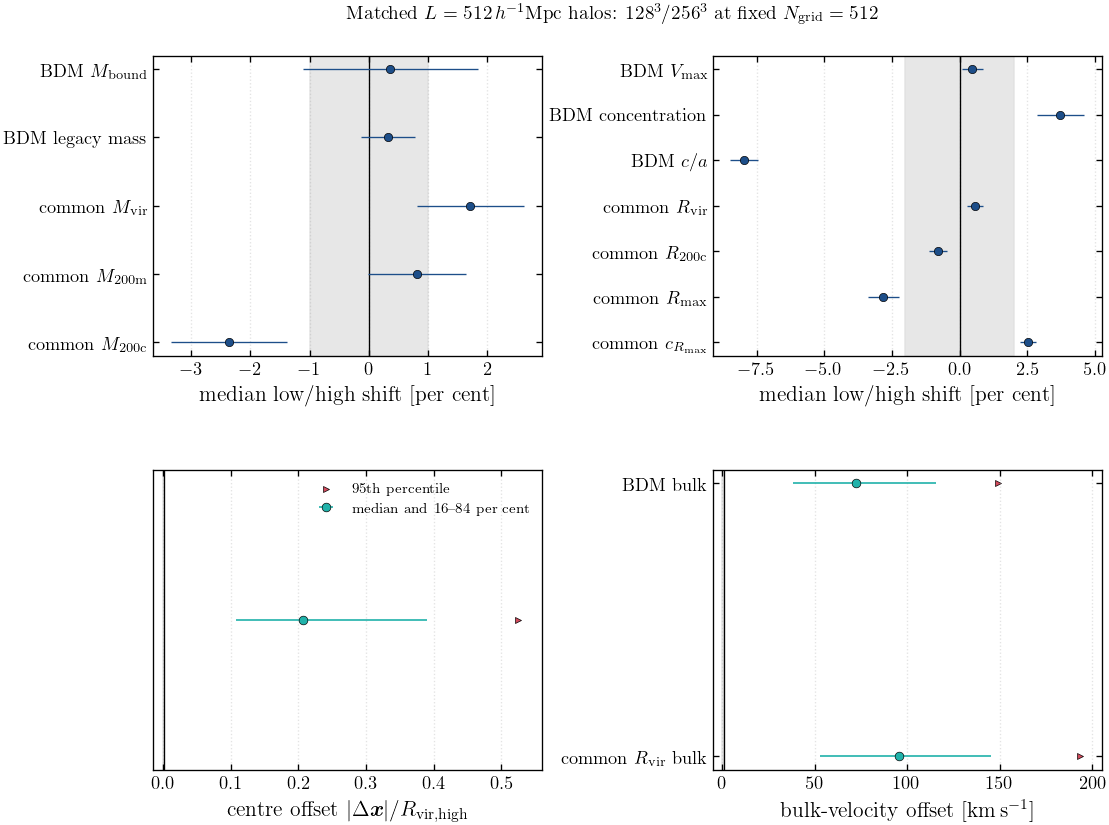
\includegraphics[width=\linewidth,height=0.58\textheight,keepaspectratio]{figs/cluster_tail_matched_properties.png}
    \end{column}
    \hfill
    \begin{column}{0.33\textwidth}
      \begin{phasebox}[top=0.9mm,bottom=0.9mm]{bdmblue}
        {\color{bdmblue}\bfseries L512 cluster-tail control}\par\smallskip
        \footnotesize
        $128^3/256^3$ particles at fixed $N_{\rm grid}=512$;
        786 reciprocal matches at the common mass cut.
      \end{phasebox}

      \vspace{0.4ex}
      \scriptsize
      \begin{tabularx}{\linewidth}{@{}Xr@{}}
        common $M_{200\mathrm c}$ & $-2.37\%$ \\
        BDM concentration & $+3.72\%$ \\
        BDM $c/a$ & $-7.95\%$ \\
        centre offset & $0.2075\,R_{\rm vir}$ \\
        BDM bulk offset & $72.2\,\mathrm{km\,s^{-1}}$ \\
        common-$R_{\rm vir}$ bulk offset & $95.5\,\mathrm{km\,s^{-1}}$ \\
      \end{tabularx}

      \vspace{0.4ex}
      \begin{phasebox}[colback=bdmrose!6,top=0.8mm,bottom=0.8mm]{bdmrose}
        \scriptsize
        Particle resolution: sensitive (three phases). Pure force resolution:
        sensitive (one phase; finder mesh 512). Finder mesh: independently sensitive.
      \end{phasebox}
    \end{column}
  \end{columns}
  \source{GR, $z=0.25$; force and compact covariance retain a one-phase limitation}
\end{frame}

\begin{frame}{A separable particle--force response model fails}
  \footnotesize
  \begin{columns}[T,totalwidth=\textwidth]
    \begin{column}{0.69\textwidth}
      \centering
      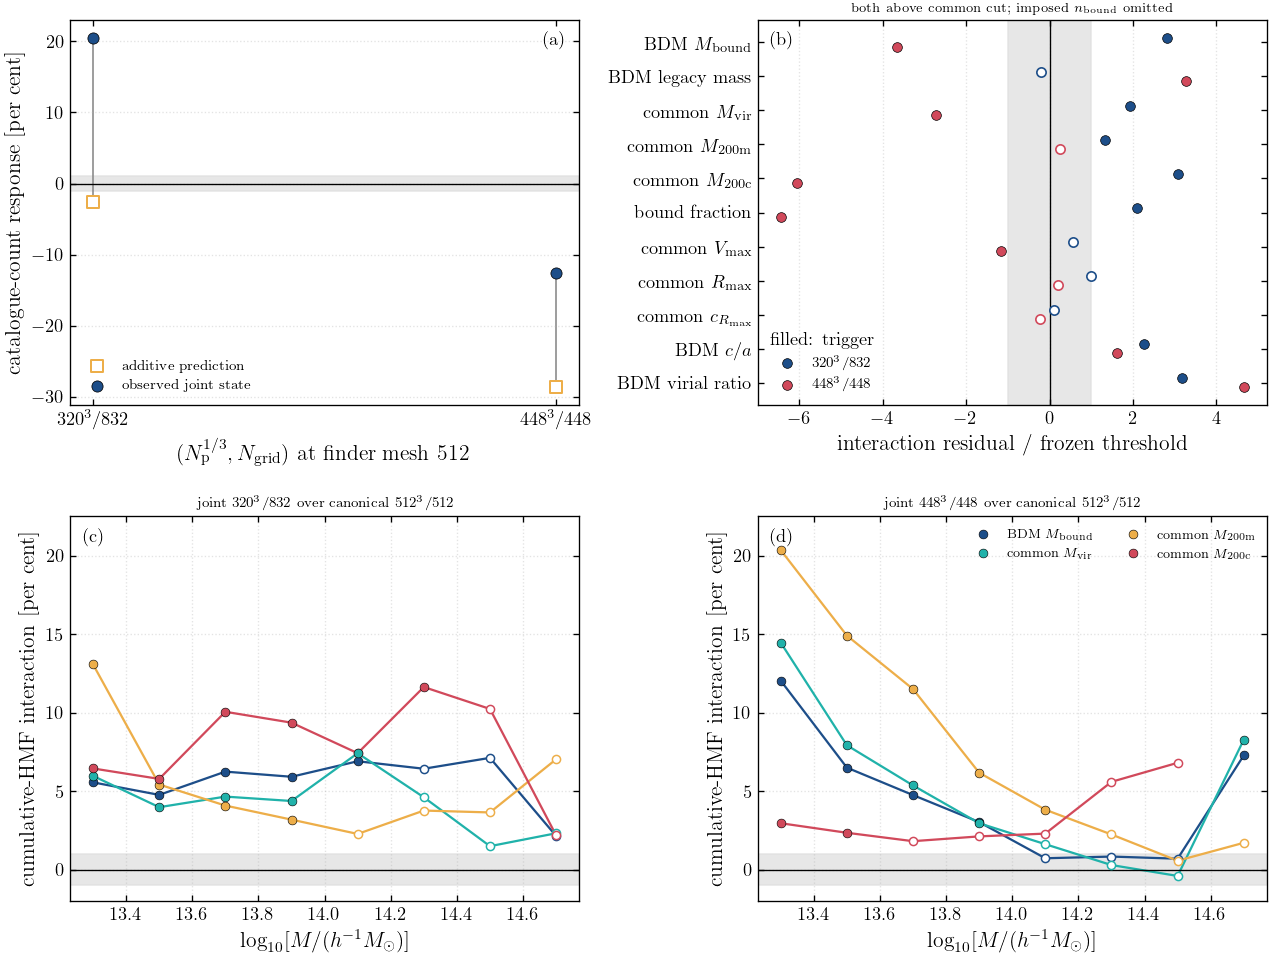
\includegraphics[width=\linewidth,height=0.55\textheight,keepaspectratio]{figs/l512_compact_joint_interactions.png}
    \end{column}
    \hfill
    \begin{column}{0.285\textwidth}
      \begin{phasebox}[colback=bdmpale,top=0.6mm,bottom=0.6mm]{bdmblue}
        \begin{tabularx}{\linewidth}{@{}>{\bfseries}l>{\raggedright\arraybackslash}X@{}}
          \color{bdmblue}22,560 & reciprocal matched halos \\
          \color{bdmrose}49/100 & physical-property triggers \\
          \color{bdmgold}51/126 & eligible HMF triggers \\
        \end{tabularx}
      \end{phasebox}

      \begin{phasebox}[top=0.6mm,bottom=0.6mm]{bdmred}
        \scriptsize
        \textbf{Catalogue-count response}\par\smallskip
        $320^3/832$: observed $+20.52\%$, additive prediction $-2.66\%$\par
        $448^3/448$: observed $-12.56\%$, additive prediction $-28.68\%$\par\smallskip
        \textbf{Largest cumulative-HMF residuals: $13.1\%$, $20.3\%$}
      \end{phasebox}
    \end{column}
  \end{columns}
  \source{Two compact points, frozen before inspection; diagnostics, not a fitted configuration}
\end{frame}

\begin{frame}{Decision: finder GO; science resolution NO-GO}
  \footnotesize
  \begin{columns}[T,totalwidth=\textwidth]
    \begin{column}{0.485\textwidth}
      \begin{phasebox}[colback=bdmgreen!7,top=1.0mm,bottom=1.0mm]{bdmgreen}
        {\color{bdmgreen}\bfseries\large GO}\par\smallskip
        Corrected canonical BDM is a numerically viable \textbf{GR finder}.
        Fast and precise builds remain viable; the bounded calibration design
        is complete.
      \end{phasebox}
    \end{column}
    \hfill
    \begin{column}{0.485\textwidth}
      \begin{phasebox}[colback=bdmred!7,top=1.0mm,bottom=1.0mm]{bdmred}
        {\color{bdmred}\bfseries\large NO-GO}\par\smallskip
        Do not select a production particle/force resolution or launch the main
        science campaign. The f(R) campaign remains deferred.
      \end{phasebox}
    \end{column}
  \end{columns}

  \vspace{0.5ex}

  \begin{columns}[T,totalwidth=\textwidth]
    \begin{column}{0.318\textwidth}
      \begin{phasebox}[top=0.9mm,bottom=0.9mm]{bdmgold}
        {\color{bdmgold}\bfseries Evidence limits}\par\smallskip
        Thresholds remain $>500$ particles. Force and compact designs have one
        phase; only $z=0.25$ was tested.
      \end{phasebox}
    \end{column}
    \hfill
    \begin{column}{0.318\textwidth}
      \begin{phasebox}[top=0.9mm,bottom=0.9mm]{bdmrose}
        {\color{bdmrose}\bfseries Unavailable controls}\par\smallskip
        No trusted external finder and no finder-specific HOD/HSM systematic
        allocation were found.
      \end{phasebox}
    \end{column}
    \hfill
    \begin{column}{0.318\textwidth}
      \begin{phasebox}[top=0.9mm,bottom=0.9mm]{bdmred}
        {\color{bdmred}\bfseries Unresolved physics}\par\smallskip
        Modified-gravity bound mass has no accepted definition; f(R) therefore
        remains deferred.
      \end{phasebox}
    \end{column}
  \end{columns}

  \vfill
  \centering
  \textbf{Next proposed simulations: 0} \quad $\vert$ \quad
  \textbf{No analytic-HMF tuning} \quad $\vert$ \quad
  \textbf{Separate error budgets}
\end{frame}

\begin{frame}{Session 4: physics changes stay opt-in until validated}
  \footnotesize
  \begin{columns}[T,totalwidth=\textwidth]
    \begin{column}{0.318\textwidth}
      \begin{phasebox}[colback=coolgray!6]{coolgray}
        {\color{coolgray}\bfseries legacy\_original}\par\smallskip
        Archived historical executable for exact reproduction only.
      \end{phasebox}
    \end{column}
    \hfill
    \begin{column}{0.318\textwidth}
      \begin{phasebox}[colback=bdmgreen!6]{bdmgreen}
        {\color{bdmgreen}\bfseries legacy\_corrected}\par\smallskip
        Session 3 safety baseline; unchanged legacy physics and schema.
      \end{phasebox}
    \end{column}
    \hfill
    \begin{column}{0.318\textwidth}
      \begin{phasebox}[colback=bdmblue!6]{bdmblue}
        {\color{bdmblue}\bfseries validated\_v1}\par\smallskip
        Explicit opt-in mode for accepted Session 4 definitions and fields.
      \end{phasebox}
    \end{column}
  \end{columns}

  \vspace{0.5ex}

  \begin{columns}[T,totalwidth=\textwidth]
    \begin{column}{0.48\textwidth}
      \begin{phasebox}[top=0.9mm,bottom=0.9mm]{bdmblue}
        {\color{bdmblue}\bfseries Evidence-backed implementation order}\par\smallskip
        \scriptsize
        \begin{enumerate}\setlength\itemsep{0em}
          \item deterministic plateaus and stable peak keys;
          \item one profile for $M_{\rm vir}$, $M_{200\rm m}$, and $M_{200\rm c}$;
          \item centre, velocity, and iterative-unbinding comparisons;
          \item periodic host flags plus resolved $V_{\max}$ and shapes;
          \item versioned catalog schema and reader migration.
        \end{enumerate}
      \end{phasebox}
    \end{column}
    \hfill
    \begin{column}{0.48\textwidth}
      \begin{phasebox}[top=0.9mm,bottom=0.9mm]{bdmteal}
        {\color{bdmteal}\bfseries Acceptance loop for every patch}\par\smallskip
        \scriptsize
        \begin{itemize}\setlength\itemsep{0em}
          \item one hypothesis and one reviewable behavior change;
          \item synthetic sentinels plus real-Fortran gates;
          \item immutable L100 cosmological comparison;
          \item reciprocal matching, HMF, exclusion, and velocity ablation;
          \item legacy identity; reject weaker invariance or definitions.
        \end{itemize}
      \end{phasebox}
    \end{column}
  \end{columns}

  \vspace{-0.3ex}
  \centering\textbf{Adopt validated physics only when its full ablation is green.}
\end{frame}

\end{document}
